\section{Results}
\label{sec:results}

\subsection{Field-deployment latency accounting for the write path}
\label{sec:results-latency-accounting}

Both transaction classes in the trace are endorsed, ordered and committed, since as Section~\ref{sec:implementation} explains every authorization outcome writes an audit entry. The interesting question is not which class is slower but how much of a write is associated with the access-control layer, and the chaincode logs a timing field on every write towards answering it: \texttt{rbac\_overhead\_ms}, recorded alongside end-to-end latency.

\subsubsection{A descriptive account, not a stage decomposition}

For each configured logical peer count, write-path latency is reported as total latency, the recorded authorization-associated span, and what is left once that span is subtracted (``remaining latency''), a plain subtraction rather than a claim that the two are independently identified Fabric stages (Limitation L1, Section~\ref{sec:limitations}).

The recorded span, averaged over the campaign at 4 peers, is \SpanLatencyPeerFour{} ms; we deliberately do not call this a direct measurement of permission-evaluation cost, since the timing field's exact instrumentation boundaries cannot be reconstructed from the deployed source (L1), and it is also larger than a complete standalone \texttt{CheckAccess} transaction, \CheckAccessMeanMs{} ms (Section~\ref{sec:latency-by-op}), because the two counters do not share a documented boundary. The remaining latency falls from \RemainingLatencyPeerFour{} ms at 4 peers to \RemainingLatencyPeerThirtyTwo{} ms at 32 peers, a \RemainingLatencyDiffFourVThirtyTwo{} ms reduction across the tested range (Table~\ref{tab:latency-table}); nothing here identifies which of ordering, validation, commit, or the peer-count-sensitive part of endorsement execution accounts for it.

\begin{table}[H]
\centering
\caption{Write-path latency accounting at 50 concurrent clients, recomputed from \texttt{raw/experiments/peer\_scaling\_transactions.csv} (run-level means, $n=8$ runs per peer count). Recorded authorization span is \texttt{rbac\_overhead\_ms}; remaining latency is total latency minus that span. Values in ms.}
\label{tab:latency-table}
\small
\begin{tabular}{lrrrr}
\toprule
Configured peers & Total latency & Recorded span & Remaining latency & Span share (\%) \\
\midrule
4 & \TotalLatencyPeerFour & \SpanLatencyPeerFour & \RemainingLatencyPeerFour & \SpanSharePeerFour \\
8 & \TotalLatencyPeerEight & \SpanLatencyPeerEight & \RemainingLatencyPeerEight & \SpanSharePeerEight \\
16 & \TotalLatencyPeerSixteen & \SpanLatencyPeerSixteen & \RemainingLatencyPeerSixteen & \SpanSharePeerSixteen \\
32 & \TotalLatencyPeerThirtyTwo & \SpanLatencyPeerThirtyTwo & \RemainingLatencyPeerThirtyTwo & \SpanSharePeerThirtyTwo \\
\bottomrule
\end{tabular}
\end{table}

\subsubsection{Recorded-span variation across configured peer counts}
\label{sec:span-variation}

Variation of the recorded span across configured peer counts is assessed descriptively. As Section~\ref{sec:peer-topology} confirms directly from the released run manifest, the campaign used \PeerRunsPerConfig{} live runs per configuration arranged as two complementary $4\times4$ Latin-square cycles, so that each configuration occupied each within-cycle position exactly twice. Across the four configured peer counts the per-configuration means span \SpanTrendSlope{} ms per doubling with a two-point-per-configuration descriptive fit ($R^2=\SpanTrendRSquared$, $p=\SpanTrendP$, $n=4$ configuration means -- necessarily low-powered); the extreme configurations (4 and 32 peers, \PeerRunsPerConfig{} runs each) differ by \SpanDiffFourVThirtyTwo{} ms with a 90\% interval of [\SpanDiffFourVThirtyTwoCINinetyLow, \SpanDiffFourVThirtyTwoCINinetyHigh] ms, entirely inside the $\pm$10\,ms margin (paired $t=\SpanDiffFourVThirtyTwoWelchT$, $p=\SpanDiffFourVThirtyTwoP$; TOST $p$\,\SpanTostP). This equivalence analysis is exploratory because the margin was selected after the data were available, rather than specified before execution.

Using the full 32-run joint regression on $\log_2(\text{peers})$ and centred run sequence (Section~\ref{sec:stats-treatment}) rather than the four configuration means, the small monotonic component in the span becomes statistically detectable ($p=\SpanLogTwoPeersJointP$) because of the larger sample, even though its magnitude ($\SpanTrendSlope$ ms per doubling) remains far inside the equivalence margin; this is a case where higher statistical power changes significance without changing practical relevance, and both results are reported rather than only the one that is easier to state. Because the span does not shrink materially when peers are added, its share of the write path rises, from \SpanSharePeerFour\% at 4 peers to \SpanSharePeerThirtyTwo\% of the smaller total at 32 peers, the opposite of what a designer would assume from the 4-peer figure alone. Splitting the remaining latency into ordering, validation, commit and the peer-count-sensitive part of endorsement needs a transaction timestamped at each Fabric hand-off, which we did not collect (L1).

\subsection{Latency by operation class}
\label{sec:latency-by-op}

Policy evaluations (\texttt{CheckAccess}, pooled across the non-write operation types recorded) average \CheckAccessMeanMs{} ms (SD \CheckAccessSdMs) and sensor writes \SensorWriteMeanMs{} ms (SD \SensorWriteSdMs, P95 \SensorWritePNinetyFiveMs, P99 \SensorWritePNinetyNineMs), a \LatencyGapMs{} ms gap between operation classes that differ simultaneously in payload size, world-state access and endorsement work; consensus is common to both, so this is not the cost of consensus. Across \RoleOpCells{} role-by-operation cells in the trace, the grant rate ranges from \GrantRateMin\% to \GrantRateMax\%; the single cell reaching \GrantRateMax\% is \texttt{Sensor|WriteSensor}, the automated field sensor-write channel rather than a human \texttt{CheckAccess} evaluation, and excluding it the remaining 35 \texttt{CheckAccess}-relevant cells cluster tightly just above \GrantRateMin\% (full 36-cell table in \texttt{analysis/outputs/02\_latency\_by\_class.json}): a trace in which the recorded operation and role determined the policy path would instead show cells near 0\% or 100\%, so these labels do not separate policy-distinct executions and do not support an operation- or privilege-specific comparison. The scripted campaign in Section~\ref{sec:results-security}, where every boundary-crossing request was refused, is the evidence that the policy itself discriminates; whether privilege level or hierarchy depth affects decision cost needs a designed experiment (Section~\ref{sec:discussion}).

\subsection{Interleaved throughput experiment}
\label{sec:results-throughput}

Figure~\ref{fig:throughput} reports throughput against offered concurrency for the HRBAC configuration and the access-control-free baseline on identical hardware and workload, recomputed from all \ThroughputRunsTotal{} live runs.

\begin{figure}[H]
\centering
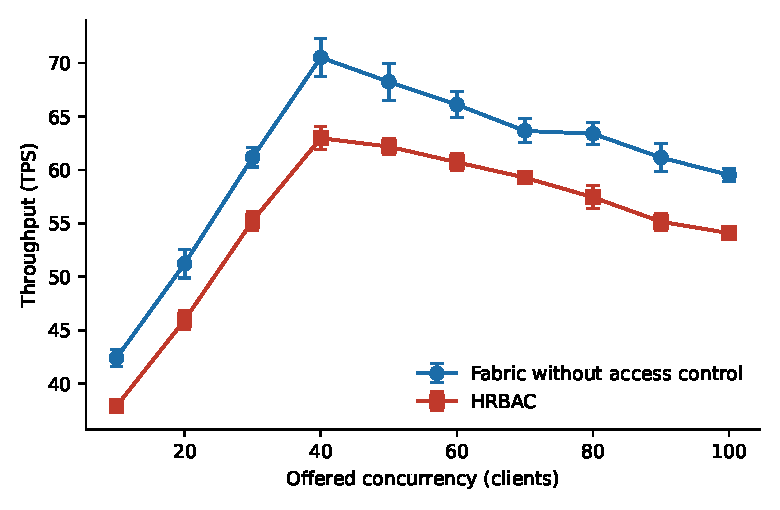
\includegraphics[width=0.85\linewidth]{../figures/figure3_throughput.pdf}
\caption{Throughput against offered concurrency for both conditions, with standard deviations over 5 live runs per condition and concurrency cell. The ten concurrency levels were tested in a single fixed ascending sequence within one session; only the two conditions were interleaved within each cell. The highest measured point (40 clients) is the observed peak under this workload; the experiment does not independently identify system capacity or the saturated resource.}
\label{fig:throughput}
\end{figure}

The primary analysis is a single factorial regression over every live run, not ten independent per-level Welch tests. Condition, centred concurrency and their interaction are fixed effects, and centred execution position within each concurrency level's 10-run cell is a covariate:
\begin{equation}
\text{TPS} \sim \text{Condition} \times \text{Concurrency}_c + \text{Position}_{\text{within cell}}.
\end{equation}
The independent experimental unit is the live run. The campaign used one experimental session rather than multiple sessions or counterbalanced blocks (Section~\ref{sec:stats-treatment}), so no session or block effect can be estimated and none is claimed. The ten concurrency levels were tested in one fixed ascending order; a run's raw campaign-wide sequence number is therefore almost collinear with concurrency ($r=\ThroughputCampaignSeqCorr$) and cannot serve as an independent order covariate. Only the two conditions were interleaved within each level.

The condition coefficient estimates the adjusted mean path difference at centred concurrency: the access-control-enabled path was \ThroughputConditionDiff{} TPS lower (95\% CI [\ThroughputConditionCILow, \ThroughputConditionCIHigh] TPS, $p$\,\ThroughputConditionP). The interaction estimates how that difference changes across the tested concurrency levels; its magnitude was \ThroughputInteractionCoef{} TPS per additional client ($p=\ThroughputInteractionP$). The within-level position effect was not detected ($p=\ThroughputPositionP$; model $R^2=\ThroughputModelRSquared$). Averaged across the ten tested concurrency levels this is a \ThroughputPctDiffMean\% reduction (SD \ThroughputPctDiffSd{} points, range \ThroughputPctDiffMin--\ThroughputPctDiffMax\%; full per-level table in \texttt{analysis/outputs/04\_throughput\_per\_level.json}). A nonsignificant interaction is not proof that the relative difference is constant outside the tested range: it means no condition-by-concurrency interaction was detected within the precision of this experiment, across ten closed-loop concurrency levels from 10 to 100 clients. All ten per-level comparisons remain significant after Holm--Bonferroni correction (\ThroughputSigAfterHolm{} of 10).

Across the tested closed-loop concurrency levels, the access-control-enabled path averaged \ThroughputPctDiffMean\% lower throughput than the comparison path. No condition-by-concurrency interaction was detected within the precision of this experiment. For the tested hardware, peer configuration, transaction semantics and closed-loop workload, the observed mean difference provides a provisional planning estimate; it should be re-estimated for other deployments and should not be interpreted as a universal authorization derating factor.

Both configurations reached their highest observed throughput at the same tested concurrency, \ThroughputBaselinePeak{} TPS for the baseline and \ThroughputHrbacPeak{} TPS for HRBAC at \ThroughputPeakLevel{} clients, after which both decline, HRBAC by \ThroughputHrbacDeclinePct\% out to 100 clients. This is the highest measured throughput under the tested closed-loop workload, not an independently established capacity ceiling; concurrency was sampled in steps of ten, so the true peak could sit anywhere in the adjacent interval, and the shared tested peak does not by itself identify which resource saturates (Limitation L3, Section~\ref{sec:limitations}) -- ordering saturation is one candidate, reported for Fabric on x86 by Thakkar et al.\ \citep{thakkar2018performance}, but so are CouchDB service times, validation and commit capacity, endorsement queueing and gateway networking, and these clients are also closed-loop, so offered concurrency is a client count rather than a controlled arrival rate. We use \emph{observed peak} throughout and do not use \emph{saturation} unless resource saturation is directly supported by telemetry, which it is not here.

\subsection{Logical peer-multiplicity experiment}
\label{sec:results-peer-scaling}

Endorsing peers are normally added to raise physical capacity. Here we increase configured logical peer multiplicity on four fixed physical hosts and observe write latency, not capacity, respond. Figure~\ref{fig:peerlatency} reports write latency as configured peer count increases from 4 to 32 at fixed offered concurrency, across \PeerRunsPerConfig{} live runs per configuration executed in the counterbalanced order confirmed in Section~\ref{sec:peer-topology}.

\begin{figure}[H]
\centering
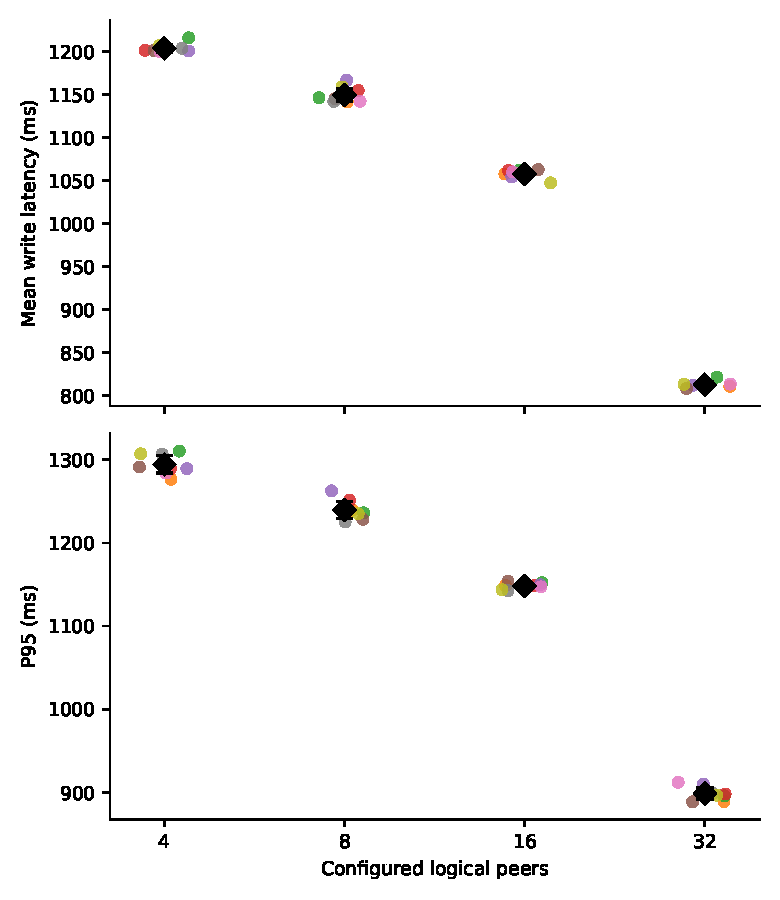
\includegraphics[width=0.78\linewidth]{../figures/figure4_peer_latency.pdf}
\caption{Write latency by configured logical peer multiplicity. Points are all \PeerRunsTotal{} run-level experimental-unit observations (colour identifies the counterbalancing block, i.e.\ repetition number), jittered horizontally on the $\log_2$ peer-count axis. Black diamonds and error bars show the group mean and 95\% confidence interval. The lower panel shows run-level P95 separately. The experiment varied logical peers on four fixed physical hosts and did not measure throughput as a function of peer count.}
\label{fig:peerlatency}
\end{figure}

Mean write latency decreased from \TotalLatencyPeerFour{} ms to \TotalLatencyPeerThirtyTwo{} ms across the tested configurations, corresponding to a 4-peer versus 32-peer difference of \TotalLatencyDiffFourVThirtyTwo{} ms (95\% CI [\TotalLatencyDiffFourVThirtyTwoCILow, \TotalLatencyDiffFourVThirtyTwoCIHigh] ms; \PeerRunsPerConfig{} live runs per configuration, paired within counterbalancing block). P95 decreased from \PNinetyFiveLatencyPeerFour{} ms to \PNinetyFiveLatencyPeerThirtyTwo{} ms, a difference of \PNinetyFiveDiffFourVThirtyTwo{} ms. The decline is close to log-linear at \LogLinearSlope{} ms per doubling with $R^2=\LogLinearRSquared$ across the four configuration means (a two-point-per-configuration descriptive fit, $p=\LogLinearP$); across the four tested configurations, the group means are approximately linear in $\log_2(\text{peer count})$, and this descriptive fit is not presented as a general scaling law. The same effect, estimated jointly with run order on all \PeerRunsTotal{} individual runs (Section~\ref{sec:stats-treatment}), remains significant at $p\,\PeerEffectPTotalLatency$ while run order does not ($p=\SeqEffectPTotalNThirtyTwo$) and the counterbalancing block effect is not detected ($p=\BlockEffectPTotalLatency$), evidence a single-run, ascending-order design could not have produced. This campaign measured latency only, not throughput, as a function of peer count (Limitation L2, Section~\ref{sec:limitations}); the separate, interleaved concurrency-throughput comparison of Section~\ref{sec:results-throughput} used a fixed peer configuration and is not informative about peer-count effects.

Every configured peer count above four is hosted on the same four physical machines as the four-peer configuration (\texttt{host\_id} is constant across all \PeerRunsTotal{} runs), so the comparison varies logical endorser multiplicity rather than genuine physical distribution (L2). Peer queue depth, proposal allocation, CPU utilisation and state-database service time were not recorded, so the experiment does not identify the mechanism. For irrigation control with a two-second responsiveness threshold \citep{leacox2013lowcost}, greater logical peer multiplicity was associated with a larger observed margin relative to that threshold in this configuration. Whether this association persists under other workloads or physical deployments remains untested.

\subsection{Revocation-stage observations}
\label{sec:revocation-results}

Revocation is where short-duration benchmark measurements are least informative, because the mechanism fires rarely and its failure mode is delay rather than error. Over the deployment, \RevocationStageRecords{} lifecycle stage records were logged across \RevocationTraceSpanDays{} days; these are stage observations rather than independent revocations, and Section~\ref{sec:revocation-audit} explains why end-to-end exposure cannot be recovered from them.

\RevocationDelayedCount{} of \RevocationStageRecords{} stage records, \RevocationDelayedPct\%, completed in a delayed state; we give the proportion without a confidence interval, since correlated stages of the same episode are not independent trials. Delayed stages are not slower on the metrics we can observe, since our timers start when publication or gossip begins and any interval spent waiting for a gateway to return is outside the measurement. Their association with recorded connectivity outages (Section~\ref{sec:availability}) motivates a reachability hypothesis, but the trace cannot determine per-episode cause or exclude the propagation protocol as a contributor (Limitation L5, Section~\ref{sec:limitations}).

The trace contains \FieldRevocationDenials{} operational access attempts recorded as denied for revocation, \FieldRevocationPerDay{} per day, spread out rather than concentrated in any single incident, kept separate from the scripted campaign of Section~\ref{sec:results-security} since one is field observation and the other synthetic testing. Because the deployment did not collect the denominator of all post-revocation access attempts, this count does not estimate the probability that a revoked credential is successfully blocked; we report it as evidence enforcement fired repeatedly in the field, not as a success rate.

\subsection{Authorization-boundary campaign}
\label{sec:results-security}

The security evaluation targets the property the system exists to provide, that no principal acts outside its role, zone or validity window. \SecurityAttemptsTotal{} scripted attempts ran, each crossing one specific boundary of the model in Section~\ref{sec:design}, organised at collection time into 8 named scenarios of 1,000 attempts each. We do not report the results by those scenario names, since repetitions of a scripted request are not independent draws from a population of attacks (no interval is attached to the block rate); the full breakdown groups every attempt by the denial mechanism actually recorded instead.

All \SecurityAttemptsTotal{} scripted requests were refused through \SecurityDenialMechanisms{} recorded denial mechanisms in the deployed implementation. We use this phrasing rather than ``all attacks were correctly refused'' because the campaign does not independently establish consistency with the intended policy, completeness of enforcement, or correctness for untested requests: expected outcomes for the role/operation dimension are checked against an oracle we built and disclose in this version (\texttt{analysis/scripts/06\_security\_oracle.py}), since the \texttt{policy-requirements.json} file an earlier draft referenced is not present in this repository (Section~\ref{sec:corrected-absent}). \OracleScoredAttempts{} of \SecurityAttemptsTotal{} attempts carry a denial reason that makes a role/operation claim (\texttt{ROLE\_INSUFFICIENT} or \texttt{OP\_NOT\_PERMITTED}); the remainder test zone, certificate, replay or intrusion-detection logic a static role/operation matrix has no opinion on. Of those \OracleScoredAttempts, \OracleConfirmed{} (\OracleConfirmedPct\%) are confirmed against the \emph{deployed} hierarchy of Section~\ref{sec:role-hierarchy}: the deployed \texttt{roles.go} agrees the attacking role lacks that permission under our disclosed operation-to-permission mapping. The remaining \OracleDiscrepant{} (\OracleDiscrepantPct\%) are not, largely because the deployed hierarchy's over-broad inheritance (Section~\ref{sec:audit-policy}) gives many roles a permission our mapping associates with the tested operation even though the request was refused by some other mechanism (zone, certificate, replay); we report this discrepancy rather than resolve it, since the corpus does not carry a separate zone- or resource-ownership attribute that would let us confirm the alternative explanation for each case. This proportion is sensitive to the operation-to-permission mapping, which is our own disclosed construction and not a value taken from the codebase (Table~\ref{tab:policy-table} note); it should not be read as a precise false-denial estimate. This extends the independent-oracle check from the role hierarchy alone to the full boundary-attempt corpus's role/operation dimension; it remains scored against \texttt{roles.go} directly for the zone, temporal, replay and identity dimensions the corpus does not separately encode, and the corpus contains no permitted (positive) requests, only denials, so no false-denial rate can be estimated from it either -- Limitation L4 is narrowed but not closed. Transport-level attacks, physical tampering and side-channel extraction are not exercised; mutual TLS and constant-time primitives address them architecturally, not empirically.

\subsection{Transmission energy and cryptographic cost}
\label{sec:energy-results}

Reliability of the residue transport is withdrawn (Section~\ref{sec:crt-audit}); what the campaign measures is cost. Per-event transmission energy falls \EnergyReductionPct\% [\EnergyReductionCILow, \EnergyReductionCIHigh] from \EnergySingleChannelMj{} mJ in single-channel mode to \EnergyCrtMj{} mJ with residue encoding ($n=150$ samples per mode), and the signing pipeline (SHA-256 \ShaTwoFiveSixMeanUs\,$\mu$s + Ed25519 sign \SignMeanUs\,$\mu$s $\approx$ \SignPipelineUs\,$\mu$s; verification \VerifyMeanUs\,$\mu$s) is negligible against the 30-minute duty cycle. This is a single-node bench measurement ($n=300$ samples per cryptographic operation) and is not generalized across all \Sensors{} devices without further instrumentation.

\subsection{Availability}
\label{sec:availability}

The online decision path, defined as reachable for all zones, was available \DecisionPathUptime\% of the deployment across \OutageCount{} single-gateway connectivity outages (\OutageMinHours--\OutageMaxHours{} h, \OutageTotalHours{} h total: a LoRa link failure, a power fluctuation and a firmware watchdog reset), with the remaining zones continuing to operate in every case; crediting gateway-hours instead of charging the whole system for one gateway's outage gives \GatewayHourUptime\%. Neither figure is a statement about request success rates, which we did not record per request, nor about data completeness: sensor writes stayed at a constant daily rate including outage days, since gateways buffer readings while disconnected and replay them on recovery, so a reading accepted after replay was authorized on replay rather than at capture time.

\subsection{Implementation-audit and deployment-postmortem results}
\label{sec:audit}

A structured code-to-specification audit conducted after deployment (Section~\ref{sec:audit-method}) identified three cross-layer defect classes -- authorization-policy deviations, invalid residue recovery and signature-verification failure -- and one revocation-observability gap that made end-to-end exposure unanswerable. We report them together because the deployed performance measurements and component-level tests did not detect them, and each was found by reading code against prose, and independently reverified for this version directly against the released source files.

\subsubsection{Authorization-policy deviations}
\label{sec:audit-policy}

The role hierarchy in \texttt{roles.go} places Certifier on the human inheritance chain rather than beside it, so Agronomist and Farmer receive \texttt{ReadAudit} through inheritance, and Certifier itself holds \texttt{ReadZone}, so an auditor could read zone sensor data directly -- the separation the introduction motivates was never in force for any of the \DeploymentDays{} days. An independent second defect is that Agronomist also holds \texttt{ControlZone} directly, inconsistent with the ``no actuation rights'' description in Section~\ref{sec:intro}. Table~\ref{tab:policy-table} lists both, together with the specified correction (Section~\ref{sec:corrected-absent}: specified and logically checked, not implemented as running chaincode in this repository).

\subsubsection{Residue-recovery bound violation}
\label{sec:crt-audit}

As Section~\ref{sec:firmware} sets out, recovery from an arbitrary pair of residues is unique only below the smallest pairwise product of the moduli, $\CrtMinBound$. The trace does not record which residue was missing when only two arrived, so a per-pair count cannot be reported. We reconstructed the packed value for all \SensorReadings{} committed readings from the released engineering-unit columns using the exact encoding in \texttt{esp32/main/main.c} (\texttt{encode\_sensor\_value}: soil count $\times$ 201 + temperature bucket). The released repository contains no calibration constant converting the released soil-moisture percentage back to the firmware's raw 12-bit ADC count, so we report the reconstruction under an explicit linear assumption and its reversed-polarity counterpart; under both, \CrtExceedPct\% of \SensorReadings{} readings exceed the smallest recovery bound -- an exhaustive count under either assumption, not an inference from the format's theoretical ceiling, though the exact packed-value minimum and maximum are calibration-dependent and reported as such in \texttt{analysis/outputs/05\_crt\_quantization.json}.

\CrtTwoResidueCount{} readings (\CrtTwoResiduePct\%) arrived with two of three residues; since every packed value here exceeded even the largest pairwise bound, each such reconstruction deterministically returned the value reduced modulo its pair's bound rather than the original, regardless of which residue was missing. All \CrtTwoResidueCount{} two-residue reconstructions are therefore mathematically incorrect, and the original cannot be recovered after the fact, since raw residue packets were not retained.

The specified correction's $\{\CrtCorrectedModuli\}$ moduli (bound $\CrtCorrectedBound$) are checked by exhaustive enumeration: every legal input to the specified 8-bit soil encoding gives a maximum packed value of $\CrtCorrectedLegalMax$, below the bound, so every value the specified encoder could produce would be uniquely recoverable. Quantising soil moisture from twelve to eight bits by bit-truncation (the natural embedded-firmware implementation, evaluated by exhaustive sweep of the 12-bit domain rather than a theoretical half-step bound) introduces a maximum error of \QuantMaxErrorPct\% of full scale (RMS \QuantRmsErrorPct\%). Whether this satisfies a particular agricultural application depends on its measurement-accuracy requirement; we do not have a manufacturer tolerance specification or calibration evidence for the deployed soil sensor to certify it in either direction.

\subsubsection{Signature-message mismatch and fail-open verification}
\label{sec:sig-audit}

The defect above would have been caught downstream had the signature path been correct; it was not. The firmware signs SHA-256 over a packed binary struct holding device identifier, reading identifier, raw soil moisture, temperature and timestamp (\texttt{esp32/main/main.c}, \texttt{sensor\_payload\_t}), but the gateway verifies an Ed25519 signature over an ASCII rendering built from the decoded value (\texttt{gateway/gateway.py}, function \texttt{\_signature\_payload}, which colon-joins the device identifier, reading identifier, decoded value and zone as text), a different message with a different byte layout and a field (zone) the firmware struct does not carry, so verification could not succeed against a genuine sensor signature. The same routine (\texttt{verify\_signature}) returns \texttt{True} immediately whenever a signature is absent (\texttt{if reading.signature is None: return True}), a fail-open default apparently intended to let the gateway run without production credentials. Both properties were confirmed by reading the two files directly, not inferred from the trace. The \SignatureValidPct\% signature-validity figure in the trace cannot mean that sensor signatures were checked and passed, and we withdraw the integrity claim rather than qualify it.

The historical firmware applies Ed25519 to the 32-byte SHA-256 digest of the packed struct, a nonstandard prehash construction retained in the historical package (Section~\ref{sec:firmware}). Matching the struct layout is therefore not sufficient by itself: a corrected verifier would need to reconstruct the canonical bytes, compute the digest, and verify the signature against that digest, matching the firmware's byte layout exactly. Such legacy-compatible corrected verification is specified but, as Section~\ref{sec:corrected-absent} states, not implemented in this repository; there is no corrected gateway verifier, no regression test, and no published byte-for-byte test vector to check it against. We do not call this a standards-based migration to Ed25519 or Ed25519ph, and no such migration is claimed or implemented.

\subsubsection{Revocation observability gap}
\label{sec:revocation-audit}

The revocation trace records lifecycle stages keyed by \texttt{event\_id}, which we confirmed maps one-to-one to \texttt{cert\_user\_id} in this trace (\texttt{analysis/scripts/07\_revocation.py}): of \RevocationSubjects{} subjects, \RevocationSubjectsAllStages{} carry all four stage types and \RevocationSubjectsOnce{} appear with only one. End-to-end exposure, the interval from revocation request to enforcement everywhere, is the quantity an operator needs, and it cannot be reconstructed from stage records alone (L5); a correlation identifier that also disambiguates repeated revocations of the same subject over the deployment window is a small change that would make it measurable.

\subsubsection{Consequences for historical data validity}

Table~\ref{tab:validity-table} states, for each audit finding, which historical results remain descriptive of the deployed implementation, which require reinterpretation, which are not measurable and which must be withdrawn. The classifications apply to the historical implementation only; they do not establish corrected-version performance (which is not evaluated, Section~\ref{sec:corrected-absent}) or the integrity of historical sensor values.

\begin{table}[H]
\centering
\caption{Validity classification of historical evidence following the implementation audit.}
\label{tab:validity-table}
\small
\begin{tabular}{p{2.6cm}p{3.6cm}p{2.0cm}p{4.4cm}}
\toprule
Historical evidence & Audit finding & Validity classification & Permitted interpretation \\
\midrule
Write-path, peer-multiplicity, throughput, cryptographic-timing and energy traces & Policy, encoding, signature and observability defects affect interpretation; corrected-code performance was not measured and no corrected code exists in this repository. & Valid for the deployed implementation & Descriptions of the historical implementation within the stated measurement boundaries; not evidence of corrected-version performance or historical sensor-value integrity. \\
Authorization decisions, denial mechanisms (Sec.~\ref{sec:results-security}) & Unintended audit inheritance and Agronomist actuation permission; the disclosed oracle mapping is our own construction, not a released file. & Reinterpreted & A record of what the deployed hierarchy enforced, not independent validation of the intended policy. \\
Sensor readings recovered from two of three residues (\CrtTwoResiduePct\%) & The legal packed-value domain exceeded every two-modulus recovery bound. & Withdrawn & Mathematically incorrect values that are not recoverable after the fact. \\
Signature-validity field & The gateway verified different bytes from those signed by the firmware and accepted missing signatures. & Withdrawn & Cannot be interpreted as evidence that sensor signatures were checked and passed. \\
Revocation end-to-end exposure & Lifecycle stages lack a within-subject episode-level correlation beyond a single event per subject in this trace. & Not measurable & Only per-stage durations are usable; episode-level exposure and causal attribution cannot be reconstructed. \\
\bottomrule
\end{tabular}
\end{table}
